%%%%%%%%%%%%%%%%%%%%%%%%%%%%%%%%%%%%%%%%%%%%%%%%%%%%%%%%%%%%%%%%%%%%%%%%%%%%%%%
% Copyright (C)  2015 Philipp Hacker
% Permission is granted to copy, distribute and/or modify this document
% under the terms of the GNU Free Documentation License, Version 1.3
% or any later version published by the Free Software Foundation;
% with no Invariant Sections, no Front-Cover Texts, and no Back-Cover Texts.
% A copy of the license should come with this file and/or can be obtained at
% http://www.gnu.org/licenses/fdl-1.3.html
%%%%%%%%%%%%%%%%%%%%%%%%%%%%%%%%%%%%%%%%%%%%%%%%%%%%%%%%%%%%%%%%%%%%%%%%%%%%%%%

\documentclass{beamer}
\usetheme{UniGreifswald}

\usepackage[ngerman]{babel}
\usepackage[T1]{fontenc}
\usepackage[utf8]{inputenc}

\usepackage{mathtools}
\usepackage{graphicx}
\usepackage{units}
\usepackage{siunitx}

\newcommand{\diff}{\textnormal{d}}
\newcommand{\tenpo}[1]{\cdot 10^{#1}}
\newcommand{\ix}[1]{_\text{#1}}
\newcommand{\imag}{\mathbf{i}}
\newcommand{\fett}[1]{\textbf{#1}}
\newcommand{\stichpunkt}[1]{\begin{itemize}\item #1\end{itemize}}

%%%%%%%%%%%%%%%%%%%%%%%%%%%%%%%%%%%%%%%%%%%%%%%%%%%%%%%%%%%%%%%%%%%%%%%%%%%%%%%
% BLOCKTEMPLATE
% 
% \onslide<->{
% 	\begin{frame}{}{}
% 		\begin{block}{}
% 		\onslide<->{}	
% 		\end{block}
% 	\end{frame}
% }
%%%%%%%%%%%%%%%%%%%%%%%%%%%%%%%%%%%%%%%%%%%%%%%%%%%%%%%%%%%%%%%%%%%%%%%%%%%%%%%
\title{Kinetic\ Effects\ in\ RF\ Discharges}

% \subtitle{}

\author[P. Hacker]{Philipp\ Hacker}

\date{\today}

\institute[Uni Greifswald]% (optional)
{%
	Mathematisch-Naturwissenschaftliche\ Fakultät\\%
	Institut\ für\ Physik\\%
  	Ernst-Moritz-Arndt-Universität\ Greifswald%
}

\begin{document}
%
%
%
%
% Title-Folie mit Betreuer/Gutachter:
	\begin{frame}
		\maketitle%
		\centering%
		{\scriptsize Betreuer:\ Prof.\ Dr.\ R.\ Schneider}\\%
		{\scriptsize Gutachter:\ Prof.\ Dr.\ J.\ Meichsner}%
	\end{frame}
%	
% Folie mit Inhaltsverzeichnis:
	\frame{\tableofcontents}
%
%
%
%
% Motivations-Sektion:
	\section{Motivation}
%
% Kapazitiv gekoppelte RF-Plasmen:
		\begin{frame}{Kapazitive gekopplte RF-Plasmen}
			\begin{columns}
				\column{0.45\textwidth}
					\begin{block}
						\onslide<1-5>{%
							\stichpunkt{Anwendung in Halbleiter- %
							und Computerchip-Industrie}%
						}
						\onslide<2-5>{%
							\stichpunkt{in elektronegativen %
							CCRF-Entladungen treffen schnelle Ionen %
							auf die Elektroden}%
						}
						\onslide<3-5>{%
							\stichpunkt{Oberflächenprozesse an der %
							Elektrode mit negativen Ionen}%
						}
					\end{block}
				\column{0.45\textwidth}
					\onslide<4-5>{%
						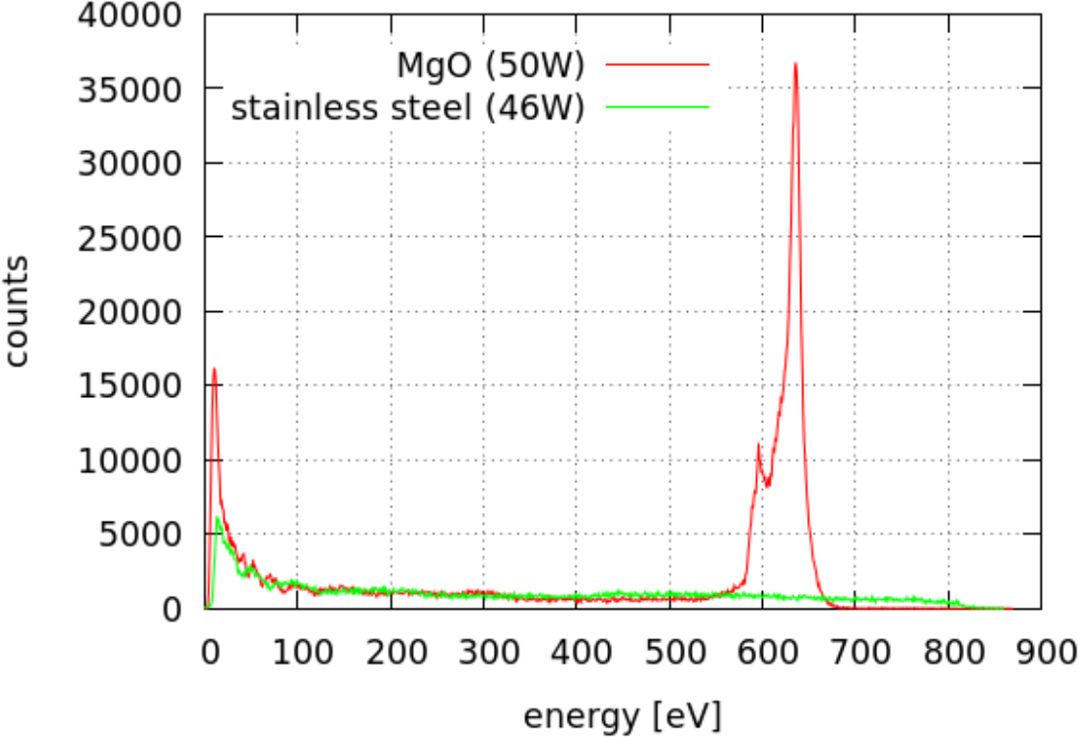
\includegraphics[width=\textwidth]{figures/niondist_material.png}	
					}
			\end{columns}
		\end{frame}
%
% Randschichteffekte:
		\begin{frame}{Randschichteffekte}
			\onslide<1>{%
				\stichpunkt{Test}%
			}
		\end{frame}
%
% Oberflaechen- und Stossprozesse:
		\begin{frame}{Oberflächen- und Stoßprozesse}
			\onslide<1>{%
				\stichpunkt{Test}%
			}
		\end{frame}
%
% Das Experiment:
	\section{Experiment}
%
		\begin{frame}{Das Experiment}
			\onslide<1>{%
				\stichpunkt{Test}%
			}
		\end{frame}
%
%
%
%
% Particle-in-Cell Simulation:
	\section{Particle-in-Cell Methode}
%
% Particle-in-Cell Simulation:
		\begin{frame}{Particle-in-Cell Methode}
			\onslide<1>{%
				\stichpunkt{Test}%
			}
		\end{frame}
%
% Monte-Carlo-Collisions:
		\begin{frame}{Monte-Carlo Stoßroutinen}
			\onslide<1>{%
				\stichpunkt{Test}%
			}
		\end{frame}
%
%
%
%
% Vergleich mit 1D Simulationen:
	\section{1D Simulation}
%
% Ergebnisse von 1D:
		\begin{frame}{1D Simulation}
			\onslide<1>{%
				\stichpunkt{Test}%
			}
		\end{frame}
%
% Energieverteilungen:
		\begin{frame}{Energieverteilungen}
			\onslide<1>{%
				\stichpunkt{Test}%
			}
		\end{frame}
%
%
% Dynamik negativer Ionen:
		\begin{frame}{Dynamik negativer Ionen}
			\onslide<1>{%
				\stichpunkt{Test}%
			}
		\end{frame}
%
%
%
%
% 2D Simulationen:
	\section{Simulationen in 2D}
%
		\begin{frame}{Simulationen in 2D}
			\onslide<1>{%
				\stichpunkt{Test}%
			}
		\end{frame}
%
% Vergleich mit 1D:
		\begin{frame}{Vergleich mit 1D}
			\onslide<1>{%
				\stichpunkt{Test}%
			}
		\end{frame}
%
% Energieverteilung negativer Ionen in 2D:
		\begin{frame}{Negative Ionen EVF}
			\onslide<1>{%
				\stichpunkt{Test}%
			}
		\end{frame}
%
% Asymmetrische Randbedingungen:
		\begin{frame}{Asymmetrische Ranbedingungen}
			\onslide<1>{%
				\stichpunkt{Test}%
			}
		\end{frame}
%
% Einfluss des Self Bias:
		\begin{frame}{Einfluss des Self Bias}
			\onslide<1>{%
				\stichpunkt{Test}%
			}
		\end{frame}
%
%
%
%
% Ausblick:
	\section{Ausblick}
%
		\begin{frame}{Ausblick}
			\onslide<1>{%
				\stichpunkt{Test}%
			}
		\end{frame}
%
%
\end{document}
